\documentclass{ximera}  


%\usepackage{todonotes}
%\usepackage{mathtools} %% Required for wide table Curl and Greens
%\usepackage{cuted} %% Required for wide table Curl and Greens
\newcommand{\todo}{}

\usepackage{esint} % for \oiint
\ifxake%%https://math.meta.stackexchange.com/questions/9973/how-do-you-render-a-closed-surface-double-integral
\renewcommand{\oiint}{{\large\bigcirc}\kern-1.56em\iint}
\fi


\graphicspath{
  {./}
  {jpg}
  {ximeraTutorial/}
  {basicPhilosophy/}
  {functionsOfSeveralVariables/}
  {normalVectors/}
  {lagrangeMultipliers/}
  {vectorFields/}
  {greensTheorem/}
  {shapeOfThingsToCome/}
  {dotProducts/}
  {partialDerivativesAndTheGradientVector/}
  {../productAndQuotientRules/exercises/}
  {../motionAndPathsInSpace/exercises/}
  {../normalVectors/exercisesParametricPlots/}
  {../continuityOfFunctionsOfSeveralVariables/exercises/}
  {../partialDerivativesAndTheGradientVector/exercises/}
  {../directionalDerivativeAndChainRule/exercises/}
  {../commonCoordinates/exercisesCylindricalCoordinates/}
  {../commonCoordinates/exercisesSphericalCoordinates/}
  {../greensTheorem/exercisesCurlAndLineIntegrals/}
  {../greensTheorem/exercisesDivergenceAndLineIntegrals/}
  {../shapeOfThingsToCome/exercisesDivergenceTheorem/}
  {../greensTheorem/}
  {../shapeOfThingsToCome/}
  {../separableDifferentialEquations/exercises/}
  {vectorFields/}
}

\newcommand{\mooculus}{\textsf{\textbf{MOOC}\textnormal{\textsf{ULUS}}}}

\usepackage{tkz-euclide}\usepackage{tikz}
\usepackage{tikz-cd}
\usetikzlibrary{arrows}
\tikzset{>=stealth,commutative diagrams/.cd,
  arrow style=tikz,diagrams={>=stealth}} %% cool arrow head
\tikzset{shorten <>/.style={ shorten >=#1, shorten <=#1 } } %% allows shorter vectors

\usetikzlibrary{backgrounds} %% for boxes around graphs
\usetikzlibrary{shapes,positioning}  %% Clouds and stars
\usetikzlibrary{matrix} %% for matrix
\usepgfplotslibrary{polar} %% for polar plots
\usepgfplotslibrary{fillbetween} %% to shade area between curves in TikZ
\usetkzobj{all}
\usepackage[makeroom]{cancel} %% for strike outs
%\usepackage{mathtools} %% for pretty underbrace % Breaks Ximera
%\usepackage{multicol}
\usepackage{pgffor} %% required for integral for loops



%% http://tex.stackexchange.com/questions/66490/drawing-a-tikz-arc-specifying-the-center
%% Draws beach ball
\tikzset{pics/carc/.style args={#1:#2:#3}{code={\draw[pic actions] (#1:#3) arc(#1:#2:#3);}}}



\usepackage{array}
\setlength{\extrarowheight}{+.1cm}
\newdimen\digitwidth
\settowidth\digitwidth{9}
\def\divrule#1#2{
\noalign{\moveright#1\digitwidth
\vbox{\hrule width#2\digitwidth}}}





\newcommand{\RR}{\mathbb R}
\newcommand{\R}{\mathbb R}
\newcommand{\N}{\mathbb N}
\newcommand{\Z}{\mathbb Z}

\newcommand{\sagemath}{\textsf{SageMath}}


%\renewcommand{\d}{\,d\!}
\renewcommand{\d}{\mathop{}\!d}
\newcommand{\dd}[2][]{\frac{\d #1}{\d #2}}
\newcommand{\pp}[2][]{\frac{\partial #1}{\partial #2}}
\renewcommand{\l}{\ell}
\newcommand{\ddx}{\frac{d}{\d x}}

\newcommand{\zeroOverZero}{\ensuremath{\boldsymbol{\tfrac{0}{0}}}}
\newcommand{\inftyOverInfty}{\ensuremath{\boldsymbol{\tfrac{\infty}{\infty}}}}
\newcommand{\zeroOverInfty}{\ensuremath{\boldsymbol{\tfrac{0}{\infty}}}}
\newcommand{\zeroTimesInfty}{\ensuremath{\small\boldsymbol{0\cdot \infty}}}
\newcommand{\inftyMinusInfty}{\ensuremath{\small\boldsymbol{\infty - \infty}}}
\newcommand{\oneToInfty}{\ensuremath{\boldsymbol{1^\infty}}}
\newcommand{\zeroToZero}{\ensuremath{\boldsymbol{0^0}}}
\newcommand{\inftyToZero}{\ensuremath{\boldsymbol{\infty^0}}}



\newcommand{\numOverZero}{\ensuremath{\boldsymbol{\tfrac{\#}{0}}}}
\newcommand{\dfn}{\textbf}
%\newcommand{\unit}{\,\mathrm}
\newcommand{\unit}{\mathop{}\!\mathrm}
\newcommand{\eval}[1]{\bigg[ #1 \bigg]}
\newcommand{\seq}[1]{\left( #1 \right)}
\renewcommand{\epsilon}{\varepsilon}
\renewcommand{\phi}{\varphi}


\renewcommand{\iff}{\Leftrightarrow}

\DeclareMathOperator{\arccot}{arccot}
\DeclareMathOperator{\arcsec}{arcsec}
\DeclareMathOperator{\arccsc}{arccsc}
\DeclareMathOperator{\si}{Si}
\DeclareMathOperator{\scal}{scal}
\DeclareMathOperator{\sign}{sign}


%% \newcommand{\tightoverset}[2]{% for arrow vec
%%   \mathop{#2}\limits^{\vbox to -.5ex{\kern-0.75ex\hbox{$#1$}\vss}}}
\newcommand{\arrowvec}[1]{{\overset{\rightharpoonup}{#1}}}
%\renewcommand{\vec}[1]{\arrowvec{\mathbf{#1}}}
\renewcommand{\vec}[1]{{\overset{\boldsymbol{\rightharpoonup}}{\mathbf{#1}}}\hspace{0in}}

\newcommand{\point}[1]{\left(#1\right)} %this allows \vector{ to be changed to \vector{ with a quick find and replace
\newcommand{\pt}[1]{\mathbf{#1}} %this allows \vec{ to be changed to \vec{ with a quick find and replace
\newcommand{\Lim}[2]{\lim_{\point{#1} \to \point{#2}}} %Bart, I changed this to point since I want to use it.  It runs through both of the exercise and exerciseE files in limits section, which is why it was in each document to start with.

\DeclareMathOperator{\proj}{\mathbf{proj}}
\newcommand{\veci}{{\boldsymbol{\hat{\imath}}}}
\newcommand{\vecj}{{\boldsymbol{\hat{\jmath}}}}
\newcommand{\veck}{{\boldsymbol{\hat{k}}}}
\newcommand{\vecl}{\vec{\boldsymbol{\l}}}
\newcommand{\uvec}[1]{\mathbf{\hat{#1}}}
\newcommand{\utan}{\mathbf{\hat{t}}}
\newcommand{\unormal}{\mathbf{\hat{n}}}
\newcommand{\ubinormal}{\mathbf{\hat{b}}}

\newcommand{\dotp}{\bullet}
\newcommand{\cross}{\boldsymbol\times}
\newcommand{\grad}{\boldsymbol\nabla}
\newcommand{\divergence}{\grad\dotp}
\newcommand{\curl}{\grad\cross}
%\DeclareMathOperator{\divergence}{divergence}
%\DeclareMathOperator{\curl}[1]{\grad\cross #1}
\newcommand{\lto}{\mathop{\longrightarrow\,}\limits}

\renewcommand{\bar}{\overline}

\colorlet{textColor}{black}
\colorlet{background}{white}
\colorlet{penColor}{blue!50!black} % Color of a curve in a plot
\colorlet{penColor2}{red!50!black}% Color of a curve in a plot
\colorlet{penColor3}{red!50!blue} % Color of a curve in a plot
\colorlet{penColor4}{green!50!black} % Color of a curve in a plot
\colorlet{penColor5}{orange!80!black} % Color of a curve in a plot
\colorlet{penColor6}{yellow!70!black} % Color of a curve in a plot
\colorlet{fill1}{penColor!20} % Color of fill in a plot
\colorlet{fill2}{penColor2!20} % Color of fill in a plot
\colorlet{fillp}{fill1} % Color of positive area
\colorlet{filln}{penColor2!20} % Color of negative area
\colorlet{fill3}{penColor3!20} % Fill
\colorlet{fill4}{penColor4!20} % Fill
\colorlet{fill5}{penColor5!20} % Fill
\colorlet{gridColor}{gray!50} % Color of grid in a plot

\newcommand{\surfaceColor}{violet}
\newcommand{\surfaceColorTwo}{redyellow}
\newcommand{\sliceColor}{greenyellow}




\pgfmathdeclarefunction{gauss}{2}{% gives gaussian
  \pgfmathparse{1/(#2*sqrt(2*pi))*exp(-((x-#1)^2)/(2*#2^2))}%
}


%%%%%%%%%%%%%
%% Vectors
%%%%%%%%%%%%%

%% Simple horiz vectors
\renewcommand{\vector}[1]{\left\langle #1\right\rangle}


%% %% Complex Horiz Vectors with angle brackets
%% \makeatletter
%% \renewcommand{\vector}[2][ , ]{\left\langle%
%%   \def\nextitem{\def\nextitem{#1}}%
%%   \@for \el:=#2\do{\nextitem\el}\right\rangle%
%% }
%% \makeatother

%% %% Vertical Vectors
%% \def\vector#1{\begin{bmatrix}\vecListA#1,,\end{bmatrix}}
%% \def\vecListA#1,{\if,#1,\else #1\cr \expandafter \vecListA \fi}

%%%%%%%%%%%%%
%% End of vectors
%%%%%%%%%%%%%

%\newcommand{\fullwidth}{}
%\newcommand{\normalwidth}{}



%% makes a snazzy t-chart for evaluating functions
%\newenvironment{tchart}{\rowcolors{2}{}{background!90!textColor}\array}{\endarray}

%%This is to help with formatting on future title pages.
\newenvironment{sectionOutcomes}{}{}



%% Flowchart stuff
%\tikzstyle{startstop} = [rectangle, rounded corners, minimum width=3cm, minimum height=1cm,text centered, draw=black]
%\tikzstyle{question} = [rectangle, minimum width=3cm, minimum height=1cm, text centered, draw=black]
%\tikzstyle{decision} = [trapezium, trapezium left angle=70, trapezium right angle=110, minimum width=3cm, minimum height=1cm, text centered, draw=black]
%\tikzstyle{question} = [rectangle, rounded corners, minimum width=3cm, minimum height=1cm,text centered, draw=black]
%\tikzstyle{process} = [rectangle, minimum width=3cm, minimum height=1cm, text centered, draw=black]
%\tikzstyle{decision} = [trapezium, trapezium left angle=70, trapezium right angle=110, minimum width=3cm, minimum height=1cm, text centered, draw=black]




 
\title{Waves on Transmission Lines} 
\author{Milica Markovic} 
\outcome{Apply phasor transformation to a time-domain equation to obtain frequency-domain equation.}
\begin{document}  
\begin{abstract}  

\end{abstract}  
\maketitle    





\section{Standing Waves}


In the previous section we introduced the voltage reflection
coefficient that relates the forward to reflected voltage phasor.


\begin{eqnarray}
\Gamma = \frac{\tilde{V}_0^-}{\tilde{V}_0^+} = \frac{Z_L -Z_0}{Z_L +Z_0} \label{reflcoe}
\end{eqnarray}


If we substitute Equation \ref{reflcoe} to Eq.\ref{vtl11} we get for the voltage wave

\begin{eqnarray}
\tilde{V}(z) = \tilde{V}_0^+ e^{-j \beta z} +\tilde{V}_0^- e^{j \beta z} \label{vtl11}\\
\tilde{V}(z) = \tilde{V}_0^+ e^{-j \beta z} + \Gamma  \tilde{V}_0^+ e^{j \beta z} \nonumber
\\
\tilde{V}(z)= \tilde{V}_0^+ (e^{-j \beta z} - \Gamma  e^{j \beta z}  ) \label{vtl01}
\end{eqnarray}

since $\Gamma = |\Gamma| e^{j \Theta_r}$ Eq.\ref{vtl01} becomes


\begin{eqnarray}
\tilde{V}(z)= \tilde{V}_0^+ (e^{-j \beta z} - |\Gamma|  e^{j \beta z + \Theta_r}  ) \label{vtl011}
\end{eqnarray}



and for the current wave



\begin{eqnarray}
I(z) = \frac{\tilde{V}_0^+}{Z_0} e^{-j \beta z} -  \frac{\tilde{V}_0^-}{Z_0} e^{j \beta z} \label{ctl1}\\
I(z) =  \frac{\tilde{V}_0^+}{Z_0}  e^{-j \beta z} + \Gamma \frac{\tilde{V}_0^+}{Z_0}  e^{j \beta z} \nonumber
\\
I(z)=   \frac{\tilde{V}_0^+}{Z_0}  (e^{-j \beta z} - \Gamma  e^{j \beta z}  ) \label{ctl01}
\end{eqnarray}

The voltage and the current waveform on a transmission line are
therefore given by Eqns.\ref{vtl01}, \ref{ctl01}. Now we have two
equations and one unknown $\tilde{V}_0^+$! We will solve these two equations
in Lecture 7. Now let's look at the physical meaning of these
equations.


In Eq.\ref{vtl01}, $\Gamma$ is the voltage reflection coefficient,
$\tilde{V}_0^+$ is the phasor of the forward going wave, $z$ is the axis in
the direction of wave propagation, $\beta$ is the phase
constant\footnote{imaginary part of the complex propagation constant},
$Z_0$ is the impedance of the transmission line\footnote{defined as
the ratio of forward going voltage and current}. $\tilde{V}(z)$ is a complex
number, phasor. We will find the magnitude and phase of the voltage on
the transmission line.




The magnitude of a complex number can be found as $|z|=\sqrt{z
z^*}$.

\begin{eqnarray}
|\tilde{V}(z)|=\sqrt{\tilde{V}(z) \tilde{V}(z)^*} \nonumber  \\
|\tilde{V}(z)|=\sqrt{   \tilde{V}_0^+ (e^{-j \beta z} - |\Gamma|  e^{j \beta z +
 \Theta_r}  )  
   \tilde{V}_0^+ (e^{j \beta z} - |\Gamma|  e^{-(j \beta z + \Theta_r)}     )} \nonumber
\\
|\tilde{V}(z)|= \tilde{V}_0^+ \sqrt{(e^{-j \beta z} - |\Gamma|  e^{j \beta z +
|\Theta_r}  )  
  (e^{j \beta z} - |\Gamma|  e^{-(j \beta z + \Theta_r)}     )}
\nonumber \\
|\tilde{V}(z)|= \tilde{V}_0^+ \sqrt{1+  |\Gamma|  e^{-(2j \beta z +
|\Theta_r)}    + |\Gamma|  e^{j 2 \beta z + \Theta_r} +|\Gamma|^2     )}
\nonumber \\
|\tilde{V}(z)|= \tilde{V}_0^+ \sqrt{1+ |\Gamma|^2 + |\Gamma| ( e^{-(2j \beta z +
 \Theta_r)}   +  e^{(j 2 \beta z + \Theta_r)}     )}
 \nonumber \\
|\tilde{V}(z)|= \tilde{V}_0^+  \sqrt{1+ |\Gamma|^2 + 2 |\Gamma| \cos(2 \beta z +\Theta_r)} \label{sw1} 
\end{eqnarray}

The magnitude of the total voltage on the transmission line is given
by Eq.\ref{sw1}. It seems like a complicated function.

\begin{itemize}
 \item Let's start 
from a simple case when the voltage reflection coefficient on the
tranmission line is $\Gamma=0$ and draw the magnitude of the total
voltage. The magnitude is the green line in Figure \ref{flatline}. To see the movie
of this transmission line go to the class web page under Instructional Videos. Forward voltage is shown in red, reflected voltage in pink,
and the magnitude of the voltage is  green. Magnitude of the voltage is constant everywhere on the transmission line, and so the line
is called flat.




\begin{figure}[htbp]
\begin{center}
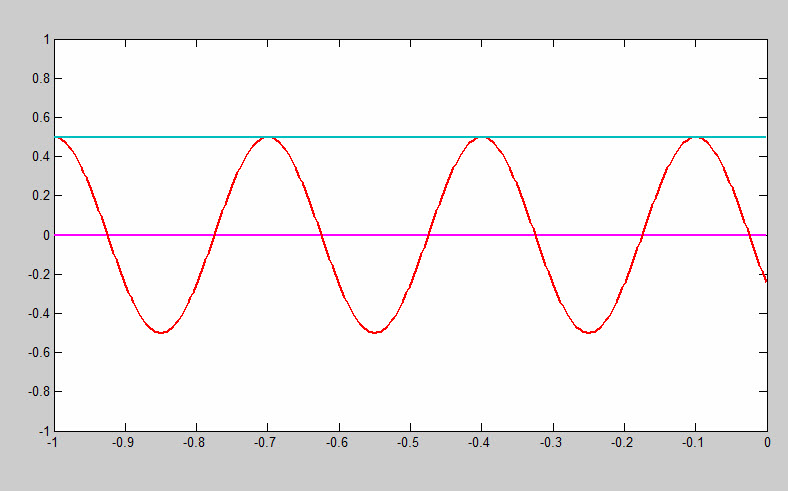
\includegraphics[scale=0.3]{../jpg/flatline.jpg}
%\strut\psfig{figure=smithchartreflection.ps,width=3cm} \\
\end{center}
\caption{Flat line.}
\label{flatline}
\end{figure}



\item Let's look at another case,  $\Gamma=0.5$ and $\Theta_r=0$. Equation \ref{swc1}  represents the magnitude of the voltage on the transmission line, and Figure \ref{reflcoeffvid} shows in green how this function looks on a transmission line. This case is shown in Figure \ref{reflcoeffvid}. 

\begin{eqnarray}
|\tilde{V}(z)|=\tilde{V}_0^+ \sqrt{\frac{5}{4}+ cos{2 \beta z} }\label{swc1}
\end{eqnarray}

\begin{figure}[htbp]
\begin{center}
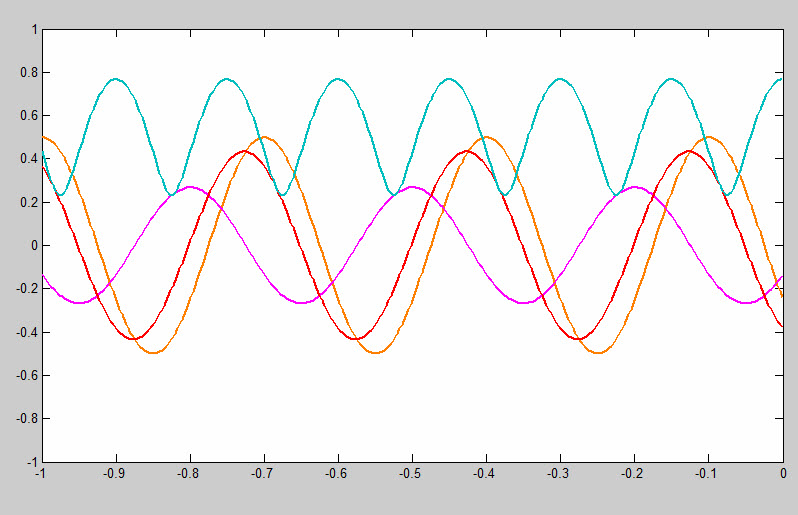
\includegraphics[scale=0.3]{specialcase.jpg}
%\strut\psfig{figure=smithchartreflection.ps,width=3cm} \\
\end{center}
\caption{Voltage on a transmission line with reflection coefficient magnitude 0.5, and zero phase.}
\label{reflcoeffvid}
\end{figure}



The function \ref{swc1} is at it's maximum 
when $cos(2 \beta z)=1$ or $z=\frac{k}{2} \lambda$, and the function
value is $\tilde{V}(z)=1.5\tilde{V}_0^+  $. It is at it's
minimum when  $cos(2 \beta z)=-1$ or $z=\frac{2 k +1}{4} \lambda$
and the function value is $\tilde{V}(z)=0.5 \tilde{V}_0^+$

It is important to mention here that the function that we see looks
like a cosine with an average value of $ \tilde{V}_0^+ $, but {\bf it is not}.
The minimums of the function are sharper then the maximums, so when
the reflection coefficient is at it's maximum of $\Gamma =1$ the
function looks like this:


\begin{figure}[htbp]
\begin{center}
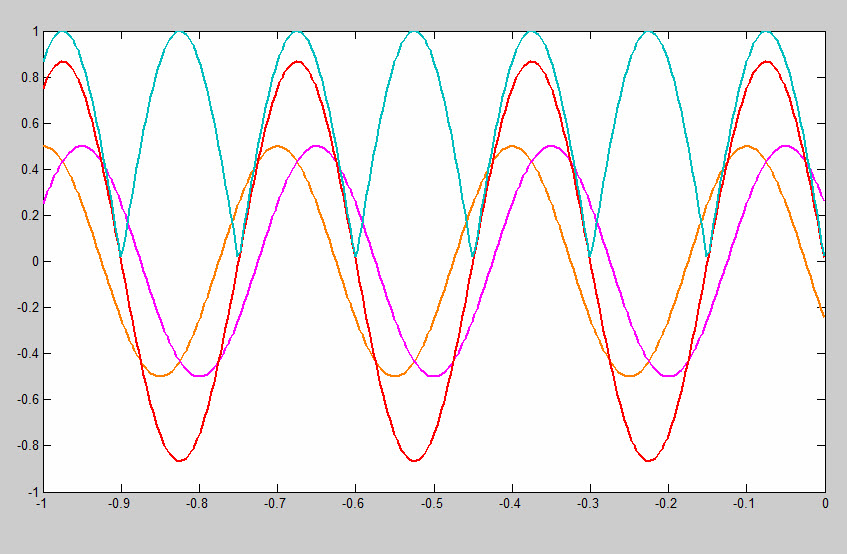
\includegraphics[scale=0.3]{../jpg/shortedline.jpg}
%\strut\psfig{figure=smithchartreflection.ps,width=3cm} \\
\end{center}
\caption{Shorted Transmission Line.}
\label{wind}
\end{figure}



\item General Case. 

In general the voltage maximums will occur when
$cos(2 \beta z)=1$

\begin{eqnarray}
|\tilde{V}(z)_{max}|=\tilde{V}_0^+\sqrt{1+|\Gamma|^2+2 |\Gamma|} \nonumber  \\
|\tilde{V}(z)_{max}| =\tilde{V}_0^+\sqrt{(1+|\Gamma|)^2}  \nonumber \\
|\tilde{V}(z)_{max}| =\tilde{V}_0^+(1+|\Gamma|) 
\end{eqnarray}



In general the voltage minimums will occur when
$cos(2 \beta z)=-1$,



\begin{eqnarray}
|\tilde{V}(z)_{min}|=\tilde{V}_0^+\sqrt{1+|\Gamma|^2-2 |\Gamma|} \nonumber  \\
|\tilde{V}(z)_{min}| =\tilde{V}_0^+\sqrt{(1-|\Gamma|)^2}  \nonumber \\
|\tilde{V}(z)_{min}| =\tilde{V}_0^+ (1-|\Gamma|) 
\end{eqnarray}

The ratio of voltage minimum on the line over the voltage maximum is
called the Voltage Standing Wave Ratio (VSWR) or just Standing Wave
Ratio (SWR).

\begin{eqnarray}
SWR=\frac{\tilde{V}(z)_{max}}{ \tilde{V}(z)_{min}} \nonumber \\
SWR=\frac{1+|\Gamma|}{1-|\Gamma|}
\end{eqnarray}

The voltage maximum position on the line is where
\begin{eqnarray}
cos(2 \beta z)=1 \nonumber \\
2 \beta z + \Theta_r = 2 n \pi \nonumber \\
z =\frac{ 2 n \pi -\Theta_r }{ 2 \beta} \nonumber \\
z=\frac{ 2 n \pi -\Theta_r }{ 4 \pi}
\end{eqnarray}



\end{itemize}

































\end{document} 
